\section{Experiment Results} \label{sec:exp_results}
Here, we present some preliminary findings. In order to explore the actual effects of \famsec on user behavior we designed a Mechanical Turk experiment where human users acted as dispatch supervisors of an autonomous vehicle (see Fig.~\ref{fig:experiment}). 

The vehicle had to complete a delivery within a given time limit as well as avoid another vehicle that could capture it. The users were trained to understand how the task would work.

\begin{figure}[tbp]
    \centering
    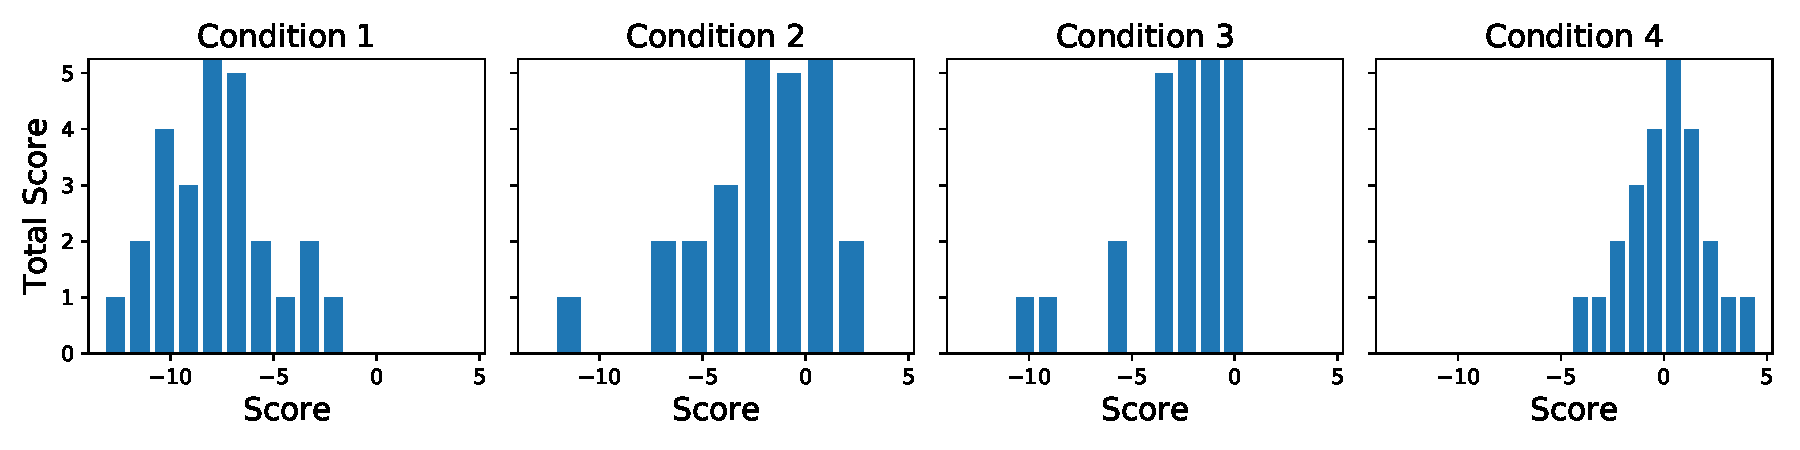
\includegraphics[width=1.0\linewidth]{Figures/test.pdf}
    \label{fig:experiment}
    \caption{Histogram of Scores From Each Condition}
\end{figure}
%
% \begin{table}[]
% \caption{Put in some statistics here---p-values}
% \label{tab:results}
% \begin{tabular}{lllll}
% \hline
% A & B & C & D \\ \cline{1-1}
% x\_Q(r=5.0) & 0.998 & 0.667 & 1.095 & 1.351 \\
% x\_Q(r=0.5) & 0.994 & 0.215 & 1.291 & 1.821 \\
% \end{tabular}
% \end{table}
